\chapter{Planificación}

\section{Fases}

El proyecto se divide en una sucesión de fases previamente establecidas que nos ayudará a estructurar, temporizar y evaluar los costes tanto económicos como humanos. Dado que el propio planteamiento del proyecto implica el uso de una serie de tecnologías como \testbf{Android} e \textbf{INDI}, y la necesidad de conocer el campo de la \textbf{astronomía}, se propuso el proyecto con bastante antelación ya que se preveía tener que realizar una fase de familiarización con las tecnologías y campos implicados. Esta fase es bastante extensa ya que se parte de cero.

\begin{itemize}
  \item \textbf{Fase 0:} Planteamiento del problema.
  \item \textbf{Fase 1:} Familiarización con las tecnologías implicadas.
  \item \textbf{Fase 2:} Especificaciones del proyecto.
  \item \textbf{Fase 3:} Análisis y diseño.
  \item \textbf{Fase 4:} Implementación.
  \item \textbf{Fase 5:} Pruebas.
  \item \textbf{Fase 6:} Documentación.
\end{itemize}

\newpage
\section{Estimación de tiempos}

A continuación se muestran las fases con sus actividades principales y la estimación inicial de tiempos.

\begin{itemize}
   \item \textbf{Planteamiento del problema:}
   \begin{itemize}
    \item Primera reunión con el cliente.
    \item Descripción de los objetivos que se persiguen.
    \item Planteamiento de las posibles tecnologías.
    \item \underline{\textit{Estimación}}: 4 horas.
    \end{itemize}
\end{itemize}

\begin{itemize}
   \item \textbf{Familiarización con las tecnologías implicadas:}
   \begin{itemize}
    \item Android: Generación de aplicaciones.
    \item Android: Generación de interfaces de usuario.
    \item Android: Posibles entornos para el desarrollador
    \item INDI: Comprensión del protocolo.
    \item INDI: Familiarización con la biblioteca \textit{``INDI for Java''}
    \item Familiarización con el campo de la astronomía.
    \item Realización de pruebas simples para estudiar la viabilidad técnica del proyecto
    \item \underline{\textit{Estimación:}} 80 horas.
   \end{itemize}
\end{itemize}

\begin{itemize}
   \item \textbf{Especificación del proyecto:}
   \begin{itemize}
    \item Tecnologías elegidas. Entornos de trabajo.
    \item Recursos humanos.
    \item Presupuesto.
    \item Temporización.
    \item \underline{\textit{Estimación:}} 18 horas.
   \end{itemize}
\end{itemize}

\begin{itemize}
   \item \textbf{Análisis y diseño:}
   \begin{itemize}
    \item Análisis de requisitos.
    \item Diagramas.
    \item Metodología de desarrollo.
    \item \underline{\textit{Estimación:}} 36 horas.
   \end{itemize}
\end{itemize}

\begin{itemize}
 \item \textbf{Implementación:}
 \begin{itemize}
  \item Herramientas seleccionadas.
  \item Creación de una aplicación en Android para abrir y cerrar conexiones de red.
  \item Creación de una aplicación en Android para conectarse con un driver INDI.
  \item Creación de una aplicación en Android para poder listar todas las propiedades y dispositivos de una conexión INDI.
  \item Creación de una aplicación en Android para poder interactuar con las propiedades de los dispositivos de una conexión INDI.
  \item Creación de una aplicación en Android para poder gestionar varias conexiones INDI simultáneamente.
  \item Creación de interfaces de usuario especificas para propiedades concretas y dispositivos concretos.
  \item \underline{\textit{Estimación:}} 180 horas.
 \end{itemize}
\end{itemize}

\begin{itemize}
 \item \textbf{Pruebas:}
 \begin{itemize}
  \item Pruebas de la aplicación en entornos simulados.
  \item Pruebas de la aplicación en entornos reales.
  \item \underline{\textit{Estimación:}} 30 horas.
 \end{itemize}
\end{itemize}

\begin{itemize}
 \item \textbf{Documentación:}
 \begin{itemize}
  \item Documentación de la aplicación.
  \item Manual de usuario.
  \item Documentación del proyecto.
  \item Manual del desarrollador.
  \item \underline{\textit{Estimación:}} 30 horas.
 \end{itemize}
\end{itemize}

\section{Recursos humanos}

Dado que el objetivo es demostrar las capacidades y competencias del alumno a la hora de afrontar un proyecto, el equipo de recursos humanos solo lo formará él, teniendo que afrontar todas las etapas del desarrollo del proyecto.
\newpage
\section{Presupuesto}

Para el presente proyecto se tendrán en cuenta los siguientes costes:

\begin{itemize}
  \item \textbf{Costes por hora de equipo humano:} En este caso son las horas dedicadas al proyecto por parte del alumno. Podemos ver que el total de horas estimadas son 298 horas. si cuantificamos el precio de desarrollo por hora. Si estimamos el precio por hora en 25\euro \ tenemos un coste en equipo humano de 7450\euro.
  \item \textbf{Costes asociados a licencias necesarias para publicar o desarrollar el software:} Dado que hemos elegido la plataforma \textbf{Android} y que basamos el proyecto en \textbf{Software Libre} no será necesario realizar ninguna inversión previa. Únicamente debemos tener en cuenta que para poder publicar la aplicación en \textit{Google Play} debemos pagar, aproximadamente, 25\euro.
  \item \textbf{Costes asociados a los entornos de prueba simulados:} Para poder realizar las pruebas ha sido necesario comprar una \textit{Raspberry Pi B+} que tiene un coste asociado de 35\euro. En ella se alojan los simuladores necesarios para testear las diferentes funciones del software.
  \item \textbf{Costes asociados a los entornos de prueba con equipos reales:} Los entornos de prueba simulados son limitados, por lo que para poder probar de forma completa el software estaría planificado adquirir instrumental astronómico. Por ello de recomienda una montura, un telescopio básico y una cámara básica por 400\euro , aunque para el proyecto este equipo ha sido prestado.
  \item \textbf{Costes asociados a la publicación y difusión a través de internet:} Para dar difusión y permitir descargar la aplicación sin tener que usar \textit{Google Play} se ha desarrollado una página web cuyo coste anual de dominio y hosting asciende a 30\euro \ al año.
\end{itemize}

\bigskip
Como puede observarse, el coste inicial del proyecto es de \textbf{7940\euro}

\section{SCRUM}

Hasta ahora hemos basado la planificación en una metodología de desarrollo clásica o \textit{en cascada}. Esta metodología se basa en un conocimiento alto de los requisitos del sistema por parte del cliente y una estructura fija y previamente establecida. 

\bigskip
Para el proyecto actual no podemos utilizar este tipo de metodología ya que el cliente solo sabe a grandes rasgos lo que quiere, dado que hay una parte de investigación asociada a la consecución del proyecto, lo cual implica la revisión de los requerimientos a lo largo del proceso de desarrollo. Es por ello que se considera más idóneo el uso de una \textbf{metodología ágil} basada en iteraciones incrementales como \textbf{Scrum}.

\bigskip
En \textbf{Scrum} se realizan entregas parciales y regulares del producto final, priorizadas por el beneficio que aportan al receptor del proyecto. Por ello, \textbf{Scrum} está especialmente indicado para proyectos en entornos complejos, donde se necesita obtener resultados pronto, donde los requisitos son cambiantes o poco definidos, donde la innovación, la competitividad, la flexibilidad y la productividad son fundamentales \cite{PASCRUM}.

\bigskip
En \textbf{Scrum} un proyecto se ejecuta en bloques temporales cortos y fijos (iteraciones de un mes natural y hasta de dos semanas, si así se necesita). Cada iteración tiene que proporcionar un resultado completo, un incremento de producto final que sea susceptible de ser entregado con el mínimo esfuerzo al cliente cuando lo solicite.

\bigskip
Debida a las características descritas, se puede aplicar al proyecto dado que en cada iteración el cliente tendrá una aplicación funcional que podrá probar y comprobar si cumple con los objetivos y que nuevos requerimientos son necesarios para, de esta forma, retroalimentar el proceso de desarrollo produciendo una nueva iteración.

\bigskip
En el la figura \ref{fig:diag_scrum} podemos ver el proceso de desarrollo por iteraciones incrementales en \textbf{Scrum}.

\begin{figure}[!ht]
  \begin{center}
  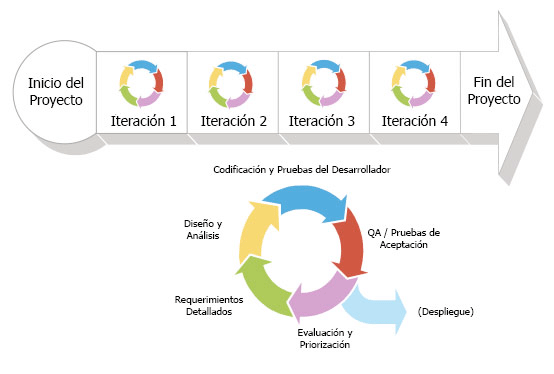
\includegraphics[width=1\textwidth]{../images/scrum-iteration-detail-es.png}
  \caption[Proceso de desarrollo Scrum]{Proceso de desarrollo Scrum (\url{http://www.qasoluciones.es/metodologia/agile})}
  \label{fig:diag_scrum}
  \end{center}
\end{figure}

Esta metodología redefine las fases en tanto en cuanto ahora debemos repetir varias veces las fases de análisis, diseño, implementación, pruebas y documentación. Las horas estimadas son las mimas ya que se repartirían entre las iteraciones. De esta forma el coste del proyecto no se ve incrementado, solo la organización de las tareas y fases de cara al desarrollo del software. 

\section{Temporización}

En la figura \ref{fig:diag_gantt_inicial} se muestra un diagrama de \textbf{Gantt}\footnote{Herramienta gráfica para mostrar la temporización de una serie de tareas} para ilustrar la temporización de las tareas basándonos en la planificación inicial. Como puede observarse, tenemos una fase inicial de planteamiento del problema. Tras ella, se realiza un parçon pactados para poder completar el resto de dociencia del curso. Después encontramos la fase de familiarización a la que se dedica 123 días para documentarse sobre los objetivos del proyecto y los campos que van a intervenir. A partir de aquí podemos encontrar la fase \textbf{Scrum} con 6 iteraciones mensuales con una reunión al inicio de cada una para el análisis de requerimientos y una final para la entrega de la versión implementada con el fin de comprobar si se han cumplido. Cuando se considera que el proyecto cumple todos los objetivos se finalizan las iteraciones y se pasa a la fase de cierre del proyecto, en paralelo con la difusión del software a través de una serie de canales de comunicación que se tratarán más a delante.

\begin{figure}[!ht]
  \begin{center}
  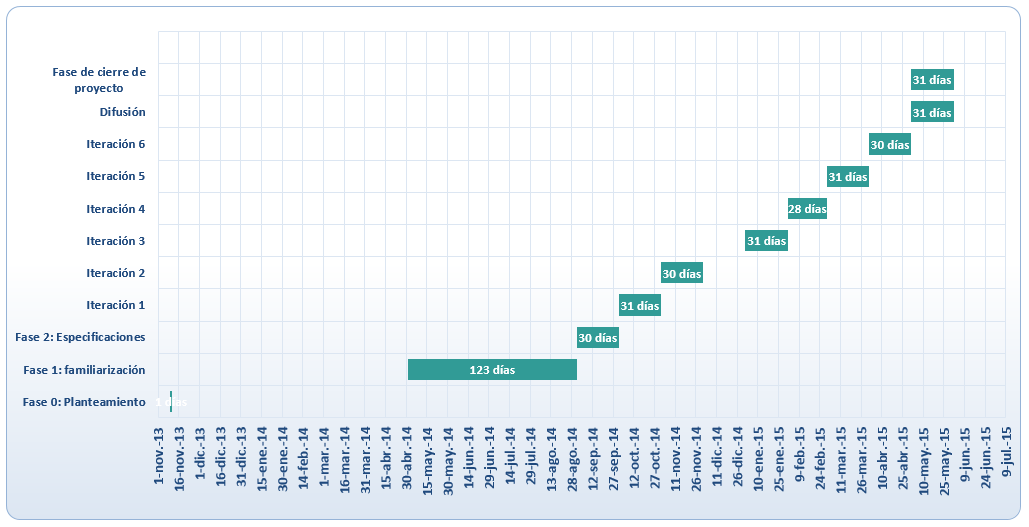
\includegraphics[width=1\textwidth]{../images/gantt_ideal.png}
  \caption{Diagrama de Gantt inicial}
  \label{fig:diag_gantt_inicial}
  \end{center}
\end{figure}

\bigskip
Aunque inicialmente se plantea una temporización basada en un número fijo de iteraciones con un periodo de un mes cada una, el proceso de desarrollo hace necesario modificar los planteamientos iniciales de horas, costes y temporización. Por ello, en la figura \ref{fig:diag_gantt_final} puede observarse una diagrama de \textbf{Gantt} con la temporización real en la que podemos ver como la fase de familiarización fue más extensa de lo previsto, debido en parte a la carga de asignaturas que impidieron dedicar más tiempo al objetivo, así como la dificultad de iniciarse en tecnologías como \textbf{Android} o \textbf{INDI}. El retraso en esta fase provocó el desplazamiento de las iteraciones. Es por ello que las dos últimas iteraciones se marcaron con una duración de 15 días para acelerar el proceso y poder entregar el proyecto en la convocatoria de septiembre. El hecho de tener que modificar una temporización planteada inicialmente es una excelente lección sobre los cálculos de tiempo y la necesidad de tener en cuenta imprevistos no contemplados inicialmente. 

\begin{figure}[!ht]
  \begin{center}
  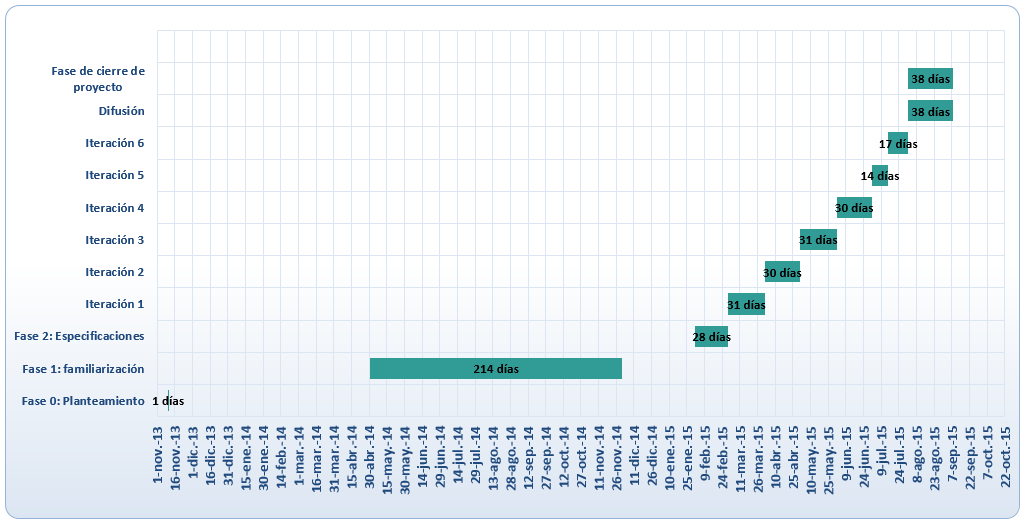
\includegraphics[width=1\textwidth]{../images/gantt_real.png}
  \caption{Diagrama de Gantt final}
  \label{fig:diag_gantt_final}
  \end{center}
\end{figure}

\begin{figure}[!ht]
  \begin{center}
  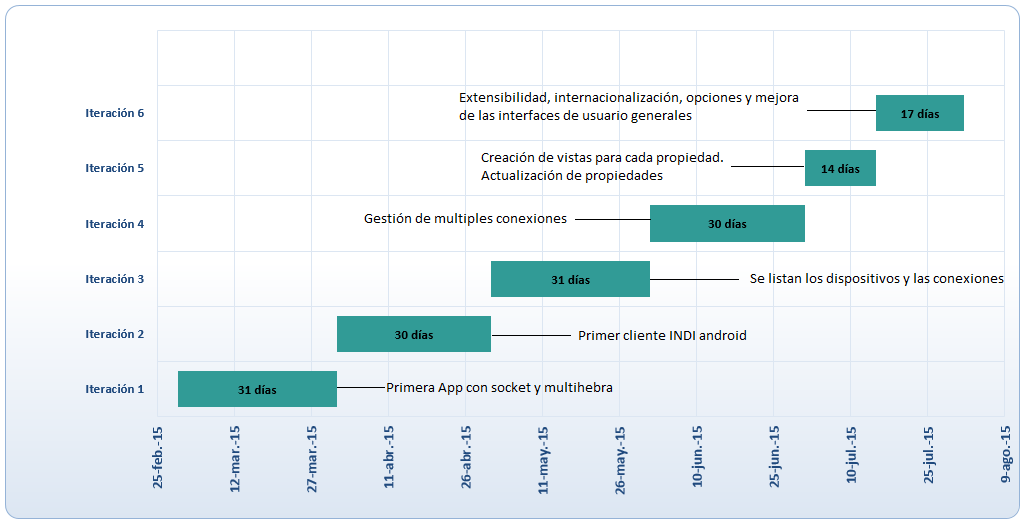
\includegraphics[width=1\textwidth]{../images/iteraciones.png}
  \caption{Diagrama de Gantt de las iteraciones}
  \label{fig:iteraciones}
  \end{center}
\end{figure}


\begin{figure}[!ht]
  \begin{center}
  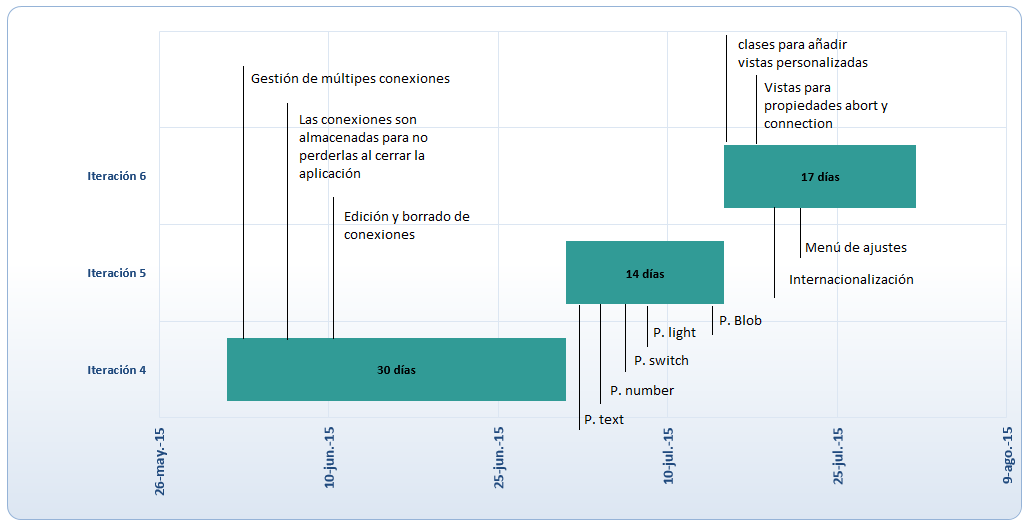
\includegraphics[width=1\textwidth]{../images/iteraciones_finales.png}
  \caption{Diagrama de Gantt de las iteraciones finales}
  \label{fig:iteraciones_finales}
  \end{center}
\end{figure}
